\selectlanguage{english}

The Standard Model of Particle Physics (SM) is, as of now, the most complete theoretical framework in subatomic physics, describing all known elementary particles and fundamental interactions \cite{Glashow-1961, Salam-1964, Weinberg-1967, Fritzsch-1972, Fritzsch-1973, Higgs-1964-1, Higgs-1964-2, Englert-1964, Guralnik-1964}, except for the very weak gravitational force. Over the last fifty years, the SM has been continuously tested via experiments, mainly in the context of particle colliders, and its validity has been confirmed by the agreement of its predictions with experimental observations, culminating in 2012 with the discovery of the Higgs boson \cite{ATLAS-2012, CMS-2012} at the Large Hadron Collider (LHC) at CERN.

Despite its success, there is strong evidence for the existence of Physics Beyond the SM (BSM): the most prominent indications include the existence of dark matter and dark energy, the observed matter-antimatter asymmetry and the non-vanishing neutrino masses. Contrary to earlier expectations, though, since its first run in 2009 the LHC has not yet detected any new particle, nor any confirmation of BSM physics: on the contrary, the huge amount of data collected in its three runs (Run 3 is currently ongoing) puts increasingly stricter exclusion limits to BSM models \cite{CMS-ATLAS-SUSY, Bsekidt-2012, Ghosh-2025, Crivellin-2015}. As a consequence, the masses of hypothesized new particles become so large that, although still not excluded, their frequent production at the LHC is hardly possible.

The lack of any observation of BSM physics at the LHC has sparked a change in the research paradigm in High-Energy Particle Physics. Substantial further increase in the energy of colliding particles at the LHC (or anywhere else) is currently not feasible, hence it is clear that BSM physics searches based on the idea of detectable resonant-like structures on top of flat backgrounds has to be supplemented by new research strategies. Indeed, new particles can still be produced at the LHC, though in a way which does not allow for their direct detection: undetected light particles could be hidden in complex final states, while heavy particles could be virtually produced for extremely short periods of time, before disappearing back into the quantum vacuum. In the latter case, these virtual particles could affect measurable properties, prompting their indirect detection as deviations from SM predictions.

Given this shift of focus towards higher experimental precision in collider physics, it is clear that reliable theoretical predictions of hadron-collision processes are needed.

\section{QCD in collider physics}

Systematic searches for BSM physics through precision studies at hadron colliders are difficult to perform, given the poorly-understood nature of the strong force which keeps hadrons together. In fact, the strong interaction is described by Quantum Chromodynamics (QCD), which has the complicated mathematical structure of a non-Abelian gauge theory (\secref{ssec:gauge-th} for details).

Although it has not been possible, so far, to describe the properties of a single proton from first principles, in the context of hadron collisions a first-principle description is made possible for a particular class of processes: hard scattering processes.

Even though hard scattering processes have a lower probability of happening, with respect, for example, to elastic scattering processes, they are of great interest to modern particle physics. To understand why, a remarkable property of non-Abelian gauge theory needs to be states: \bctxt{asymptotic freedom}. The evolution of the coupling $ \alpha(\mu^2) $ of a quantum field theory as a function of the energy scale $ \mu $ is described by the renormalization group equation (see e.g. Chapter 12 of \cite{Peskin-1995}):
\begin{equation}
  \mu^2 \frac{\dd \alpha(\mu^2)}{\dd \mu^2} = - 2 \beta(\alpha(\mu^2)) \alpha(\mu^2)
  \label{eq:ren-gr}
\end{equation}
where the $ \beta $-function has a power-series expansion like:
\begin{equation}
  \beta(\alpha) = \sum_{n \in \N_0} \beta_n \left( \frac{\alpha}{4\pi} \right)^{n+1} = \beta_0 \frac{\alpha}{4\pi} + \smo(\alpha^2)
\end{equation}
For non-Abelian gauge theories $ \beta_0 > 0 $ (for QCD, see \cite{Gross-1973, Politzer-1973}), hence the coupling becomes small at high energies (small distances). This allows for a perturbative description of hard scattering processes, which are characterized by a large momentum transfer: this kind of events happen at small distances, hence the hadronic scattering can be studied through the interaction between single partons (see \figref{fig:part-scatt}), i.e. the quarks and gluons which compose the hadrons.

\begin{figure}
  \centering
  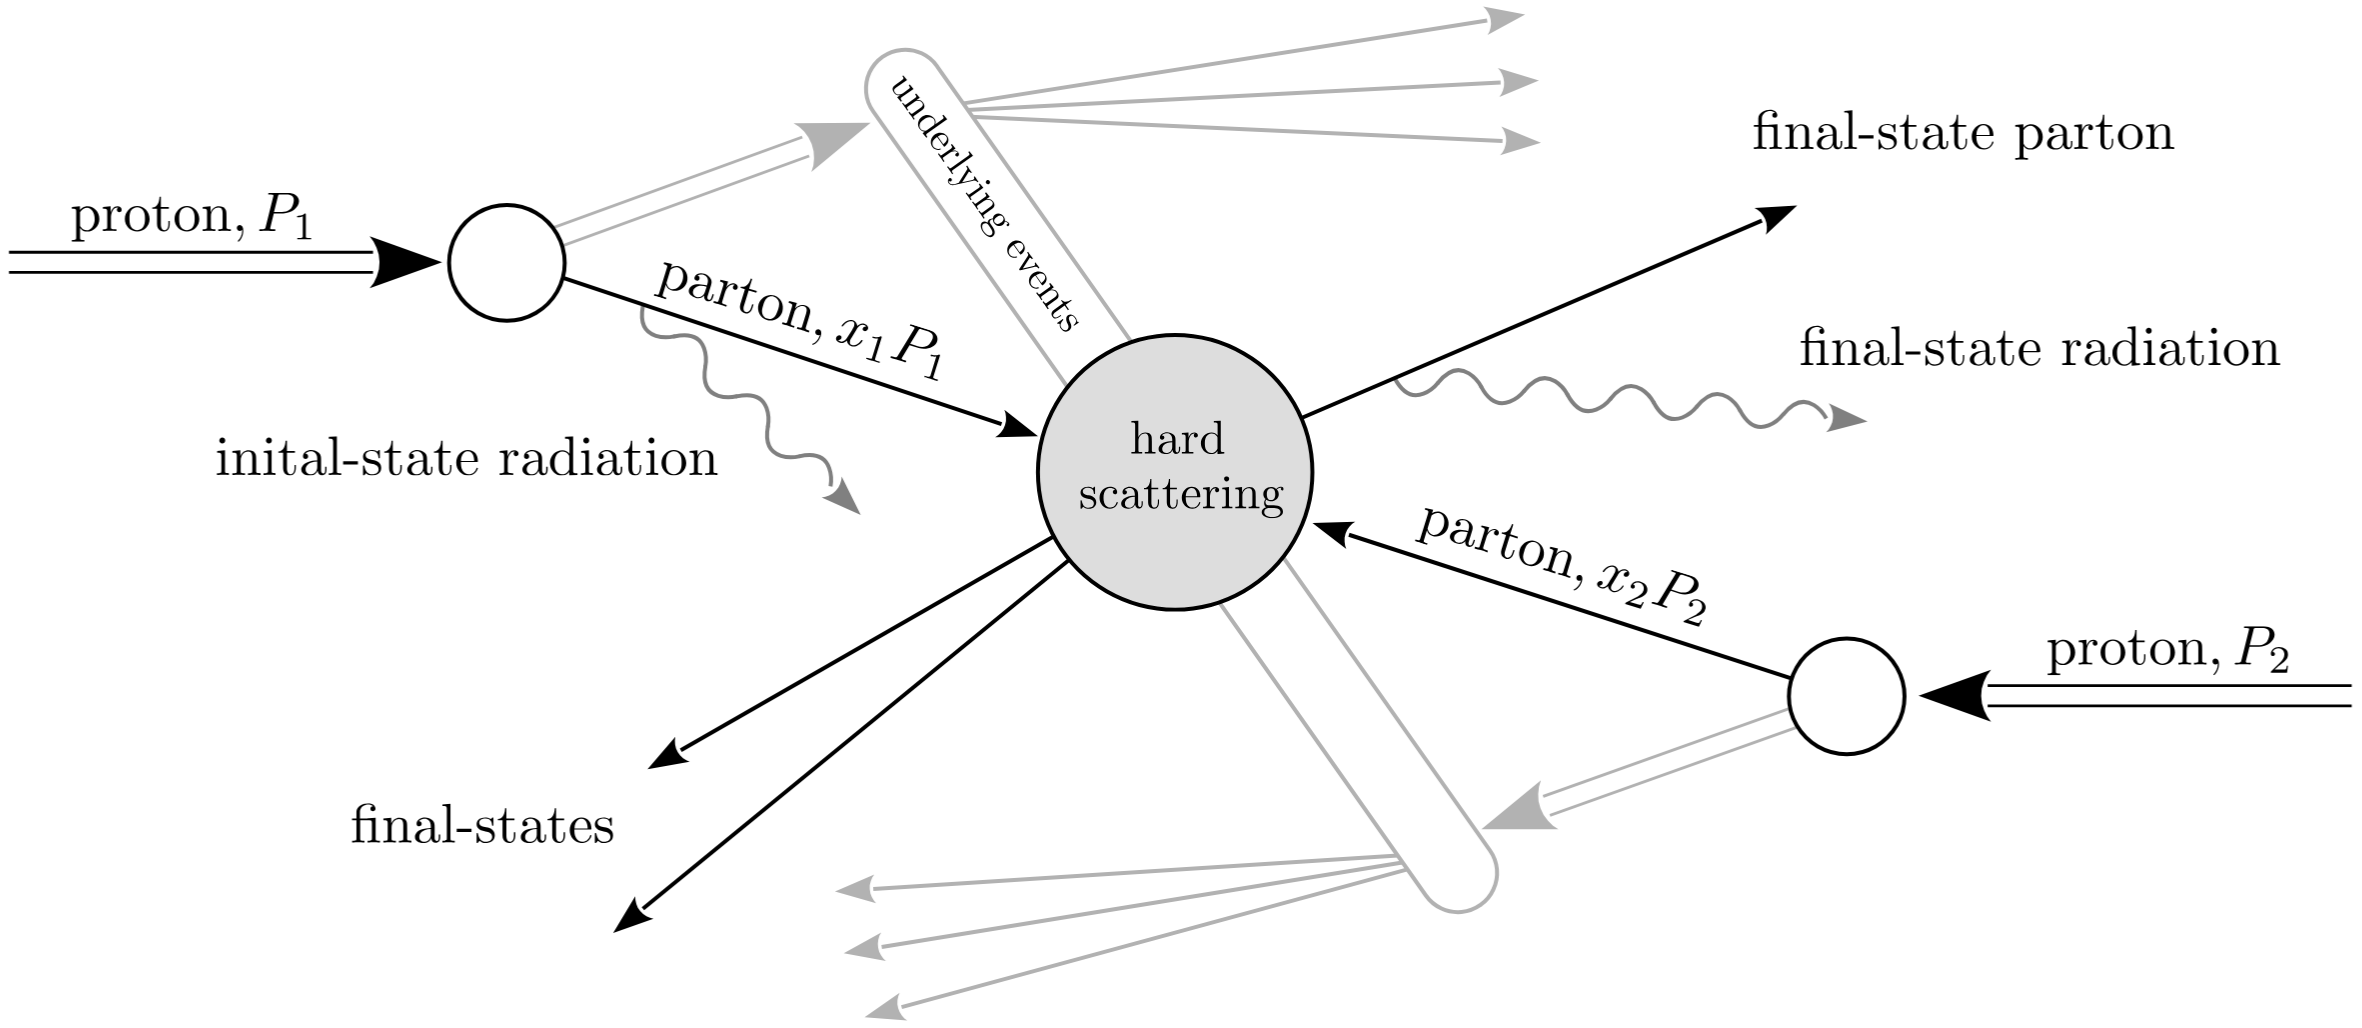
\includegraphics[width = 0.90 \textwidth]{imgs/part-scatt.png}
  \caption{Schematics of hard hadronic scattering. Due to asymptotic freedom, individual partons can be assumed to be free particles, so that their (hard) scattering can be computed via perturbative QCD. Initial- and final-state radiation accounts for beyond-leading-order effects. Figure from \cite{Asteriadis-2020}.}
  \label{fig:part-scatt}
\end{figure}

\subsection{Hadronic scattering}

Theoretical predictions for hard hadronic scattering are based on the factorization theorem \cite{Collins-1989}, which states that hadronic cross-sections can be computed from partonic cross-sections as:
\begin{equation}
  \dd\hcs_{h_1,h_2}(P_1 , P_2) = \sum_{a,b} \int_{[0,1]^2} \dd \xi_1 \dd \xi_2 \, f_a^{(h_1)}(\xi_1, \fac^2) f_b^{(h_2)}(\xi_2, \fac^2) \, \dd\pcs_{a,b}(\xi_1 P_1, \xi_2 P_2, \rc, \ren^2, \fac^2)
\end{equation}
Here, the two scattering hadrons $ h_1 , h_2 $ have momenta $ P_1 , P_2 $, while the scattering partons $ a , b $ have momentum fractions $ x_1 P_1 , x_2 P_2 $. The factorization scale $ \fac $ is taken to be equal to the renormalization scale $ \ren $ for the rest of this work.

The link between hadron-scale physics and parton-scale physics is given by \bctxt{parton distribution functions} (PDFs): in general, $ f_a^{(h)}(x) $ is the numerical probability of finding a parton $ a $ inside the hadron $ h $ with a definite energy fraction $ x : p_a = x P_h $, where $ p_a $ and $ P_h $ are the momenta of the parton and of the hadron, respectively. A crucial property of PDFs is their universality, as they are energy-independent: this means that they can be measured in a particular process and then used in many others. However, they incapsulate non-perturbative effects which are poorly understood, thus they have not been computed from first principles so far.

Another instance of non-perturbative effects arises when considering that, after the partonic interaction, final-state partons can be clustered in the so-called jets: despite the difficulty in formally defining jets (for a review of various jet algorithms, see \cite{Salam-2010}), they can intuitively be pictured as seeds of hadronic energy flow with are barely affected by non-perturbative QCD effects. While on short time-scales QCD can be treated perturbatively, on long time-scales QCD partons (and so jets too) are subject to the phenomenon of \bctxt{hadronization}.

\begin{figure}
  \centering
  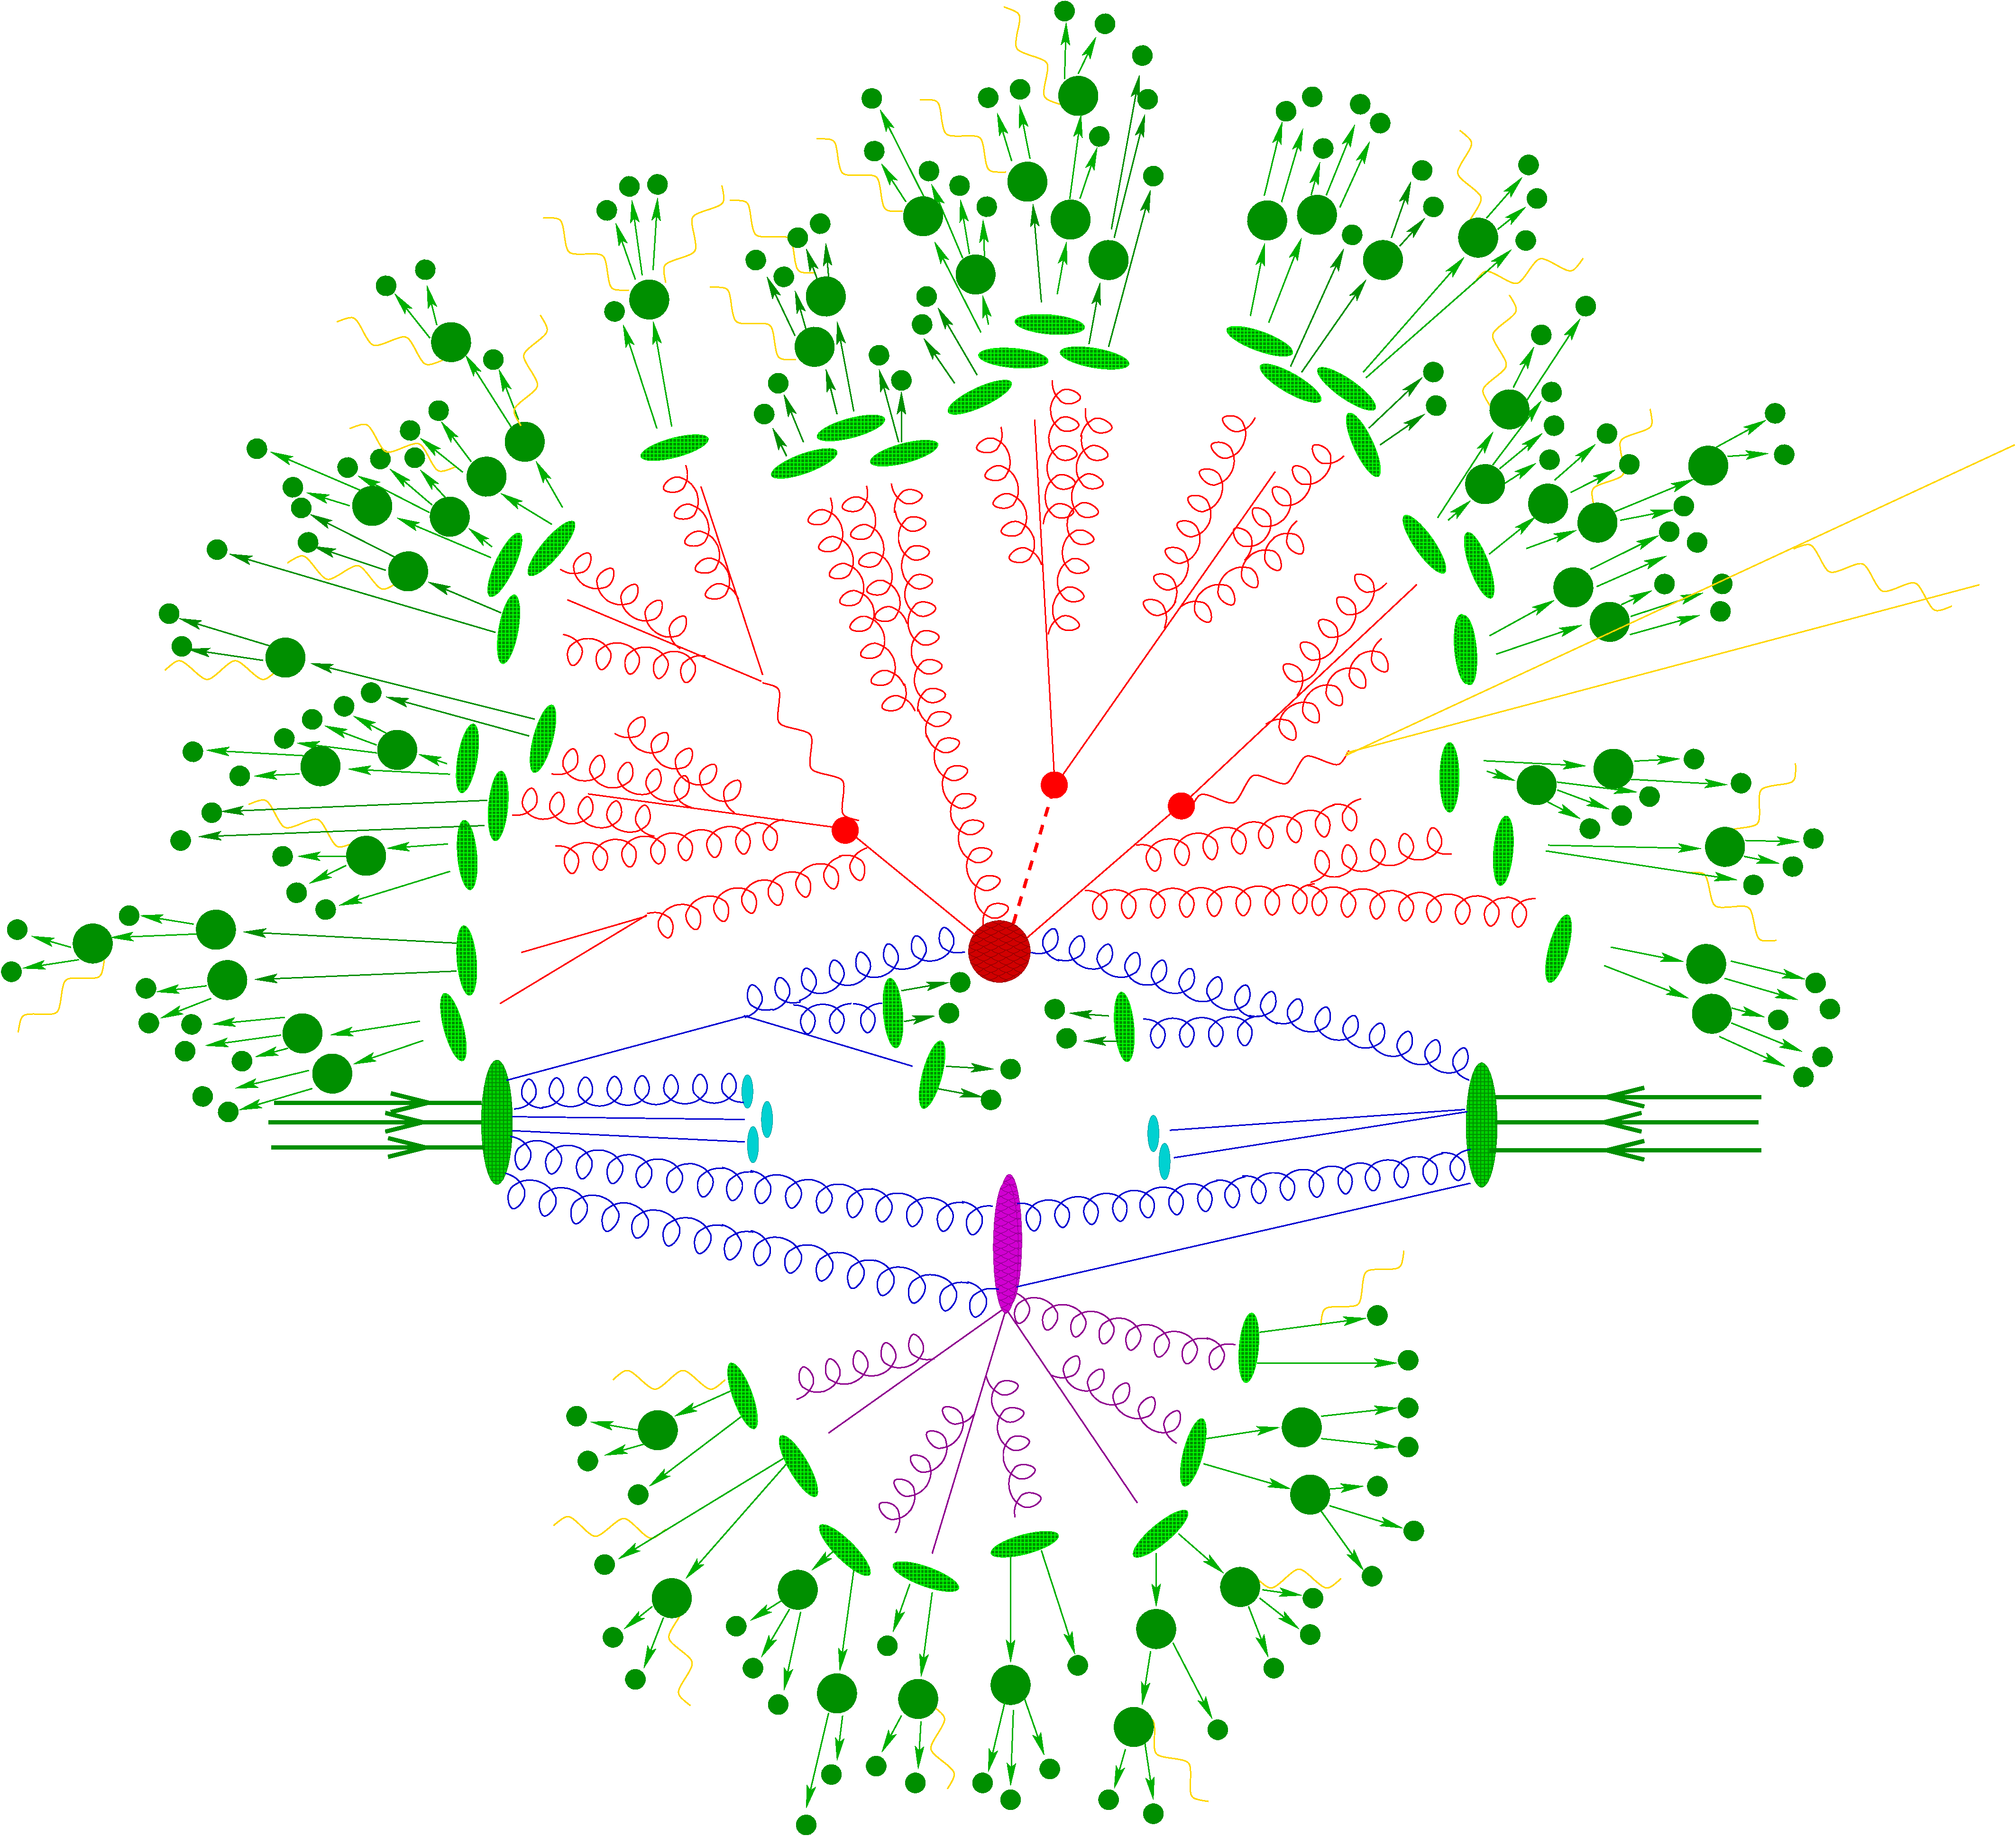
\includegraphics[width = 1.00 \textwidth]{imgs/hadr-scatt.pdf}
  \caption{Hadronization of jets produced in a hard hadronic scattering. Incoming hadrons produce initial-state radiation (blue), which determines two hard scattering events (red and purple blobs): these scatterings give rise to partonic jets (red and purple) which undergo hadronization (light green blobs), eventually decaying into heavy hadrons (dark green blobs) and soft radiation (yellow). Figure from \cite{Hoche-2014}.}
  \label{fig:hadr-scatt}
\end{figure}

Hadronization can be explained by considering a solution to \eref{eq:ren-gr}, found introducing a reference scale $ Q $:
\begin{equation}
  \rcr = \frac{\rc(Q^2)}{1 + 2 \rc(Q^2) \frac{\beta_0}{4\pi} \log \frac{\ren^2}{Q^2}}
\end{equation}
For e.g. $ \rc(m_Z^2) \approx 0.118 $ \cite{PDG-2024}. It is customary to introduce a QCD scale $ \qcd \approx 300 \mev $, so that:
\begin{equation}
  \rcr = \frac{1}{2\frac{\beta_0}{4\pi} \log \frac{\ren^2}{\qcd^2}}
\end{equation}
This expression shows that $ \ren \gg \qcd $ is the perturbative region, where asymptotic freedom makes $ \rc $ small enough for perturbative techniques. On the other hand, for $ \ren \rightarrow \qcd $ a Landau pole is present: this pole signals the breakdown of perturbation theory and the hadronization of partons, i.e. their confinement into bound states (hadrons).

As illustrated in \figref{fig:hadr-scatt}, the hard scattering process occurs at high energy $ Q \gg \qcd $ (typically $ Q \sim 1\tev $ at the LHC), resulting in jets which are unaffected by non-perturbative QCD, as their energy is well above the QCD scale; however, this energy is radiated off in the form of parton showers, and, when the threshold energy $ \qcd $ is reached, non-perturbative effects come into play, resulting in the hadronization of jets.

\subsection{Partonic scattering}

For the rest of this work, the analysis is restricted to perturbative effects only. As the partonic scattering can be treated with perturabtion theory, the partonic cross section for the scattering of two partons $ a , b $ with momenta $ p_1 , p_2 $ can be expressed as a power series in the running coupling:
\begin{equation}
  \dd\pcs_{a,b}(p_1 , p_2) = \sum_{n \in \N_0} \dd\pcs_{a,b}^{(n)}(p_1 , p_2)
\end{equation}
where each term is $ \dd\pcs^{(n)} \sim \rc^{n_0 + n} $, with $ n_0 \in \N $ giving the leading-order-dependence on $ \rcr $ due to the leading-order (LO) process, which is usually (but not always) a tree-level process.

The $ n \ge 1 $ terms form what are denoted by QCD corrections. Focusing on next-to-leading-order (NLO) corrections, they can be of two kinds: real corrections and virtual corrections. Real corrections consist in the emission of an additional parton as initial- or final-state radiation, while virtual corrections present an additional partonic loop. Examples of a real and a virtual correction to the Drell-Yan process may be:
\begin{equation*}
  \begin{tikzpicture}
    \begin{feynman}

      \vertex (a1) {\(q\)};
      \vertex[below = 3cm of a1] (a2) {\(\bar{q}\)};

      \vertex[below = 1.5cm of a1] (b1) {};
      \vertex[right = 2.25cm of b1, dot] (v1) {};

      \vertex[right = 2.25cm of v1, dot] (v2) {};
      \vertex[right = 2.25cm of v2] (b2) {};

      \vertex[above = 1.5cm of b2] (a3) {\(e^-\)};
      \vertex[below = 1.5cm of b2] (a4) {\(e^+\)};

      \vertex[dot] (c1) at ($(a1) + (1.5,-1)$) {};
      \vertex (c2) at ($(c1) + (1.5,1)$) {\(g\)};

      \diagram* {
	(a1) -- [fermion] (v1),
	(a2) -- [anti fermion] (v1),

	(v1) -- [photon, edge label = \(\gamma^*\)] (v2),

	(v2) -- [fermion] (a3),
	(v2) -- [anti fermion] (a4),

	(c1) -- [gluon] (c2),
      };
    \end{feynman}
  \end{tikzpicture}
  \qquad \qquad
  \begin{tikzpicture}
    \begin{feynman}

      \vertex (a1) {\(q\)};
      \vertex[below = 3cm of a1] (a2) {\(\bar{q}\)};

      \vertex[below = 1.5cm of a1] (b1) {};
      \vertex[right = 2.25cm of b1, dot] (v1) {};

      \vertex[right = 2.25cm of v1, dot] (v2) {};
      \vertex[right = 2.25cm of v2] (b2) {};

      \vertex[above = 1.5cm of b2] (a3) {\(e^-\)};
      \vertex[below = 1.5cm of b2] (a4) {\(e^+\)};

      \vertex[dot] (c1) at ($(a1) + (0.75,-0.5)$) {};
      \vertex[dot] (c2) at ($(a2) + (0.75,0.5)$) {};

      \diagram* {
	(a1) -- [fermion] (v1),
	(a2) -- [anti fermion] (v1),

	(v1) -- [photon, edge label = \(\gamma^*\)] (v2),

	(v2) -- [fermion] (a3),
	(v2) -- [anti fermion] (a4),

	(c1) -- [gluon, edge label' = \(g^*\)] (c2),
      };
    \end{feynman}
  \end{tikzpicture}
\end{equation*}
In general, then:
\begin{equation}
  \dd\pcs_{a,b}^{(1)}(p_1 , p_2) = \dd\pcsr_{a,b}(p_1 , p_2) + \dd\pcsv_{a,b}(p_1 , p_2) + \dd\pcspdf_{a,b}(p_1 , p_2)
\end{equation}
where $ \dd\pcsr_{a,b} $ and $ \dd\pcsv_{a,b} $ are the single-real and 1-loop corrections. The additional correction $ \dd\pcspdf_{a,b} $ is due to the collinear renormalization of PDFs.

\section{Singularities in QCD amplitudes}

show how divergences arise in the soft and collinear limits for the real case

cite UV-singularities for the virtual case (link to section about renormalization), then say that IR-singularities cancel when combined with real ones due to the kinoshita-lee-nauenberg theorem

prove the general form of collinear pdf renormalization counterterms










